\chapter{原型系统设计与实现}

    原型系统包括核心工具Lapis和用户接口两大组件. 其中, 核心工具提供从脚本解析到测试生成与执行的整套方法的原型实现. 用户接口则包括核心工具的编程API接口, 在线API脚本的上传、编辑和可视化的web应用, 以及桌面端测试管理系统. 以上各部分完全独立.

	\section{核心工具Lapis}
	
	    \begin{figure}[!htb]
	        \centering
	        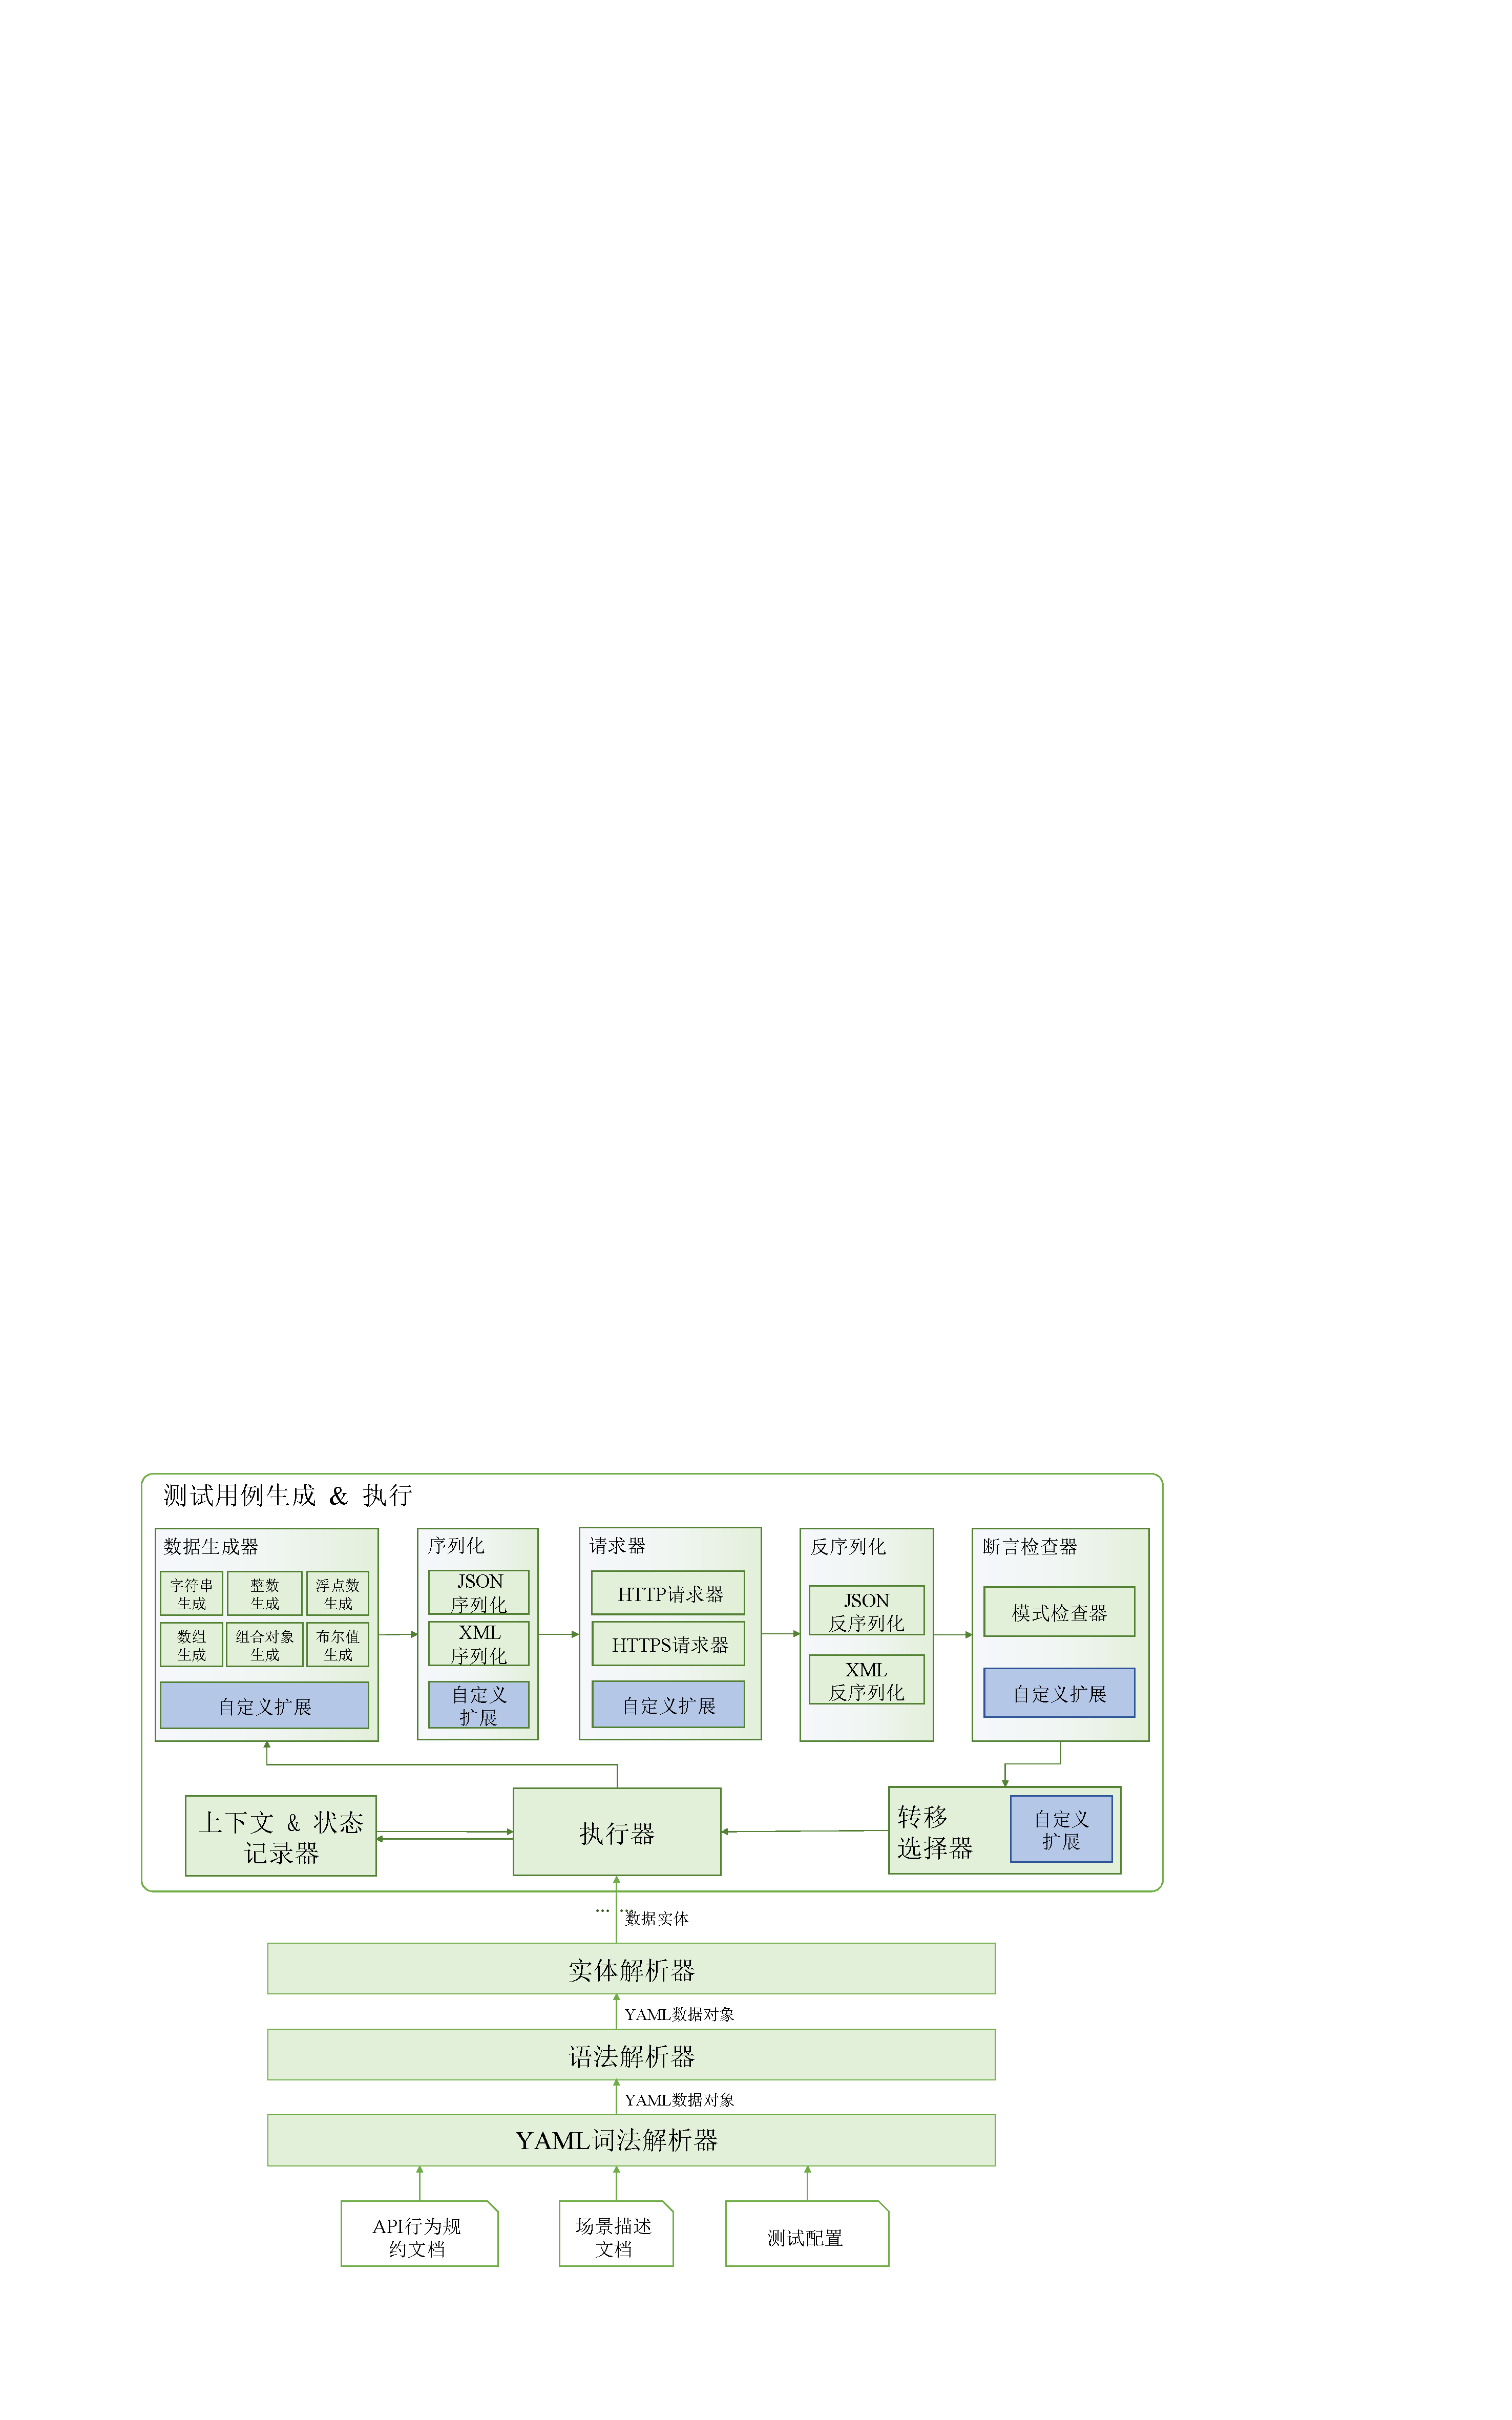
\includegraphics[width=300pt]{tool_architecture3.pdf}
	        \caption{Lapis工具整体架构. 工具的输入为API行为规约文档, 场景描述文档和测试配置. 输出为测试用例及其执行结果. 执行流从下往上, 从左往右.}
	        \label{fig:lapis_arch}
	    \end{figure}
	    
	    图\ref{fig:lapis_arch}展示了Lapis工具原型的整体架构.
	    
	    工具完全采用Python 3实现. 其依赖于一些Python开源库, 如Requests\footnote{http://docs.python-requests.org}, PyYAML\footnote{https://pyyaml.org}, rstr\footnote{https://pypi.org/project/rstr/2.1.1}, 以及标准库.
	    
	    工具的输入为三个脚本文件 - 使用OpenAPI格式描述的API行为文档, 场景模型文档, 以及测试配置文档. 本工作定义了一套格式规范, 用于表述场景模型. 测试配置文档为可选项, 内容较简单, 对API行为文档进行了少量补充, 并提供定制运行参数的功能. 三个脚本文件均为YAML格式. 它们具有着一定的层次关系: API行为文档提供了API的具体定义, 包括请求和响应的格式定义(即场景模型中状态定义的合法请求集合与合法响应集合)和请求方法, 请求URL, 请求协议等; 场景模型文档利用这些信息, 并将场景模型的状态与对应API定义关联起来, 同时为自动化测试提供具体的场景模型; 测试配置文档则提供为定义提供了补充, 并支持一些可定制选项, 如指定测试用例生成与执行的时间限制等.
	    
	    \label{sec:lapis_impl}
	    工具的输出为包含所有测试用例及其执行结果的Python列表, 列表的各个元素即为各个测试用例, 涵盖测试用例的执行序列, 生成的请求数据, 获得的响应结果, 响应时间及模型覆盖率等.

	    工具采用模块化的设计, 具有良好的可扩展性, 如图\ref{fig:lapis_arch}所示, 多个模块均支持用户自定义:
	    \begin{itemize}
	        \item 在场景模型中, 如\ref{sec:set_define}小节所述, 定义合法输入, 合法响应和转移条件可以采用自定义校验函数(对应断言检查器模块的用户扩展)和自定义生成函数(对应数据生成器模块的用户扩展);
	        \item 在请求器中, 为了支持各种不同的API服务, 除了已实现的HTTP协议API请求器和HTTPS协议API请求器外, 用户可以通过子类化抽象接口类的方法进行扩展, 通过这种方式, 可以对使用签名机制的API发送合法请求;
	        \item 在序列化模块中, 除了默认的JSON格式和XML格式序列化模块外, 用户也可以用子类化的方法, 实现自定义的序列化格式;
	        \item 在转移选择器模块中, 除了直接按转移概率随机选择转移外, 用户也可以实现接口函数并在测试配置文档中引入, 以应用启发式的算法;
	        \item 此外, 在全局测试配置中, 为了更好地与被测系统(SUT)交互, 工具提供了用于被测系统启动, 停止和序列间隔时操作的函数接口, 在测试配置文档中指定实现的函数位置, 即可引入自定义交互函数.
	    \end{itemize}  
	    自定义函数和子类的引入得益于Python的动态反射机制, 但这也要求这些自定义扩展使用Python实现.
	    
	    工具各个模块的功能如下:
	    
	    \begin{itemize}
	        \item YAML词法解析器:\\
	            此模块分析输入的三个脚本文件的格式, 分析其是否为合法YAML文档, 并建立文档树.
	        \item 语法解析器:\\
	            此模块读入数据对象, 检查每个脚本是否包括必需域以及各个域的数据合法性, 比如API行为文档中各个API参数的定义是否合法, 场景模型文档中转移的定义是否合法等.
	        \item 实体解析器:\\
	            此模块从脚本中提取出自动化测试所需信息, 而像API描述(\texttt{description}域)和开发者联系方式域(\texttt{info.contact}域)等无关域被舍去. 提取的信息使用数据实体(Python类实例)存储, 并传给测试执行器.
	        \item 测试执行器:\\
	            测试执行器调度和控制整个测试用例的生成和执行过程. 执行器也负责处理用户自定义扩展抛出的异常, 防止系统崩溃. 用户编程接口(见\ref{sec:program_interface}小节)直接与此模块进行交互.
	        \item 上下文\&状态记录器:\\
	            此模块记录测试的所有有用信息, 最后返回给用户.
	        \item 数据生成器:\\
	            此模块生成请求参数(输入数据).
	        \item 序列化:\\
	            此模块将生成的请求参数序列化/格式化为字符串.
	        \item 请求器:\\
	            此模块发送请求, 并收集响应结果. 负责处理网络交互的细节, 也可以进行自定义扩展使之支持签名机制.
	        \item 反序列化:\\
	            此模块将响应的头和响应体分离, 并根据API行为文档和测试配置文档中的数据格式定义, 从字符串解析为数据实体.
	        \item 断言检查器:\\
	            此模块对响应数据进行检查, 包括模式检查(是否符合定义的模式)和断言检查(是否满足上下文依赖和约束)两个方面.
	        \item 转移选择器:\\
	            此模块随机选择转移边, 确定当前执行序列的下一状态.
	    \end{itemize}

	\section{用户接口}
		\subsection{编程接口}
            \label{sec:program_interface}
            用户可以通过调用编程接口直接使用核心工具Lapis. 编程接口为Python函数的形式, 封装并隐藏了工具实现的具体细节. 普通用户使用\texttt{run()}函数, 即可一行完成测试生成与执行. \texttt{run()}函数的签名如下:
            \begin{flushleft}
                \scriptsize
                \tt
                \begin{lstlisting}[language=python]
def run(api_doc_path, scenario_doc_path, testconf_doc_path=None, num_case=1, verbose=0)
                \end{lstlisting}
            \end{flushleft}
            用户需要提供三个脚本文件的路径(测试配置脚本可选), 生成测试用例的总数, 以及往控制台输出信息的详细级别. 输出如\ref{sec:lapis_impl}小节所述, 为包含所有测试用例及其执行结果的Python列表.
            
		\subsection{web端脚本编辑系统}

            本文的工具与方法使用结构化的脚本文档作为输入, 脚本文档则常常需要手工撰写, 因此, 用户友好的脚本编辑和管理工具不可或缺.
            
            本工作为API行为脚本文档的编辑开发了一个在线web系统, 如图\ref{fig:frontend_screenshot}. 在此系统中, 用户可在线编辑与上传API行为脚本, 并获得解析结果的实时反馈. 如果脚本的内容合法, 前端会将所描述的API以类似于使用手册的形式进行可视化, 并展示于右栏. 为了提升可读性, 各个参数和响应体的定义采用折叠式的设计. 如果脚本的内容不合法, 系统会提示出错原因与位置. 每个注册用户拥有私有脚本文件夹, 后台记录了文件夹内各脚本的历史版本, 脚本也可从本地上传到此文件夹. 此外, 编辑系统还附带大量样例方便用户快送熟悉脚本语法.

            \begin{figure}[!htb]
                \centering
                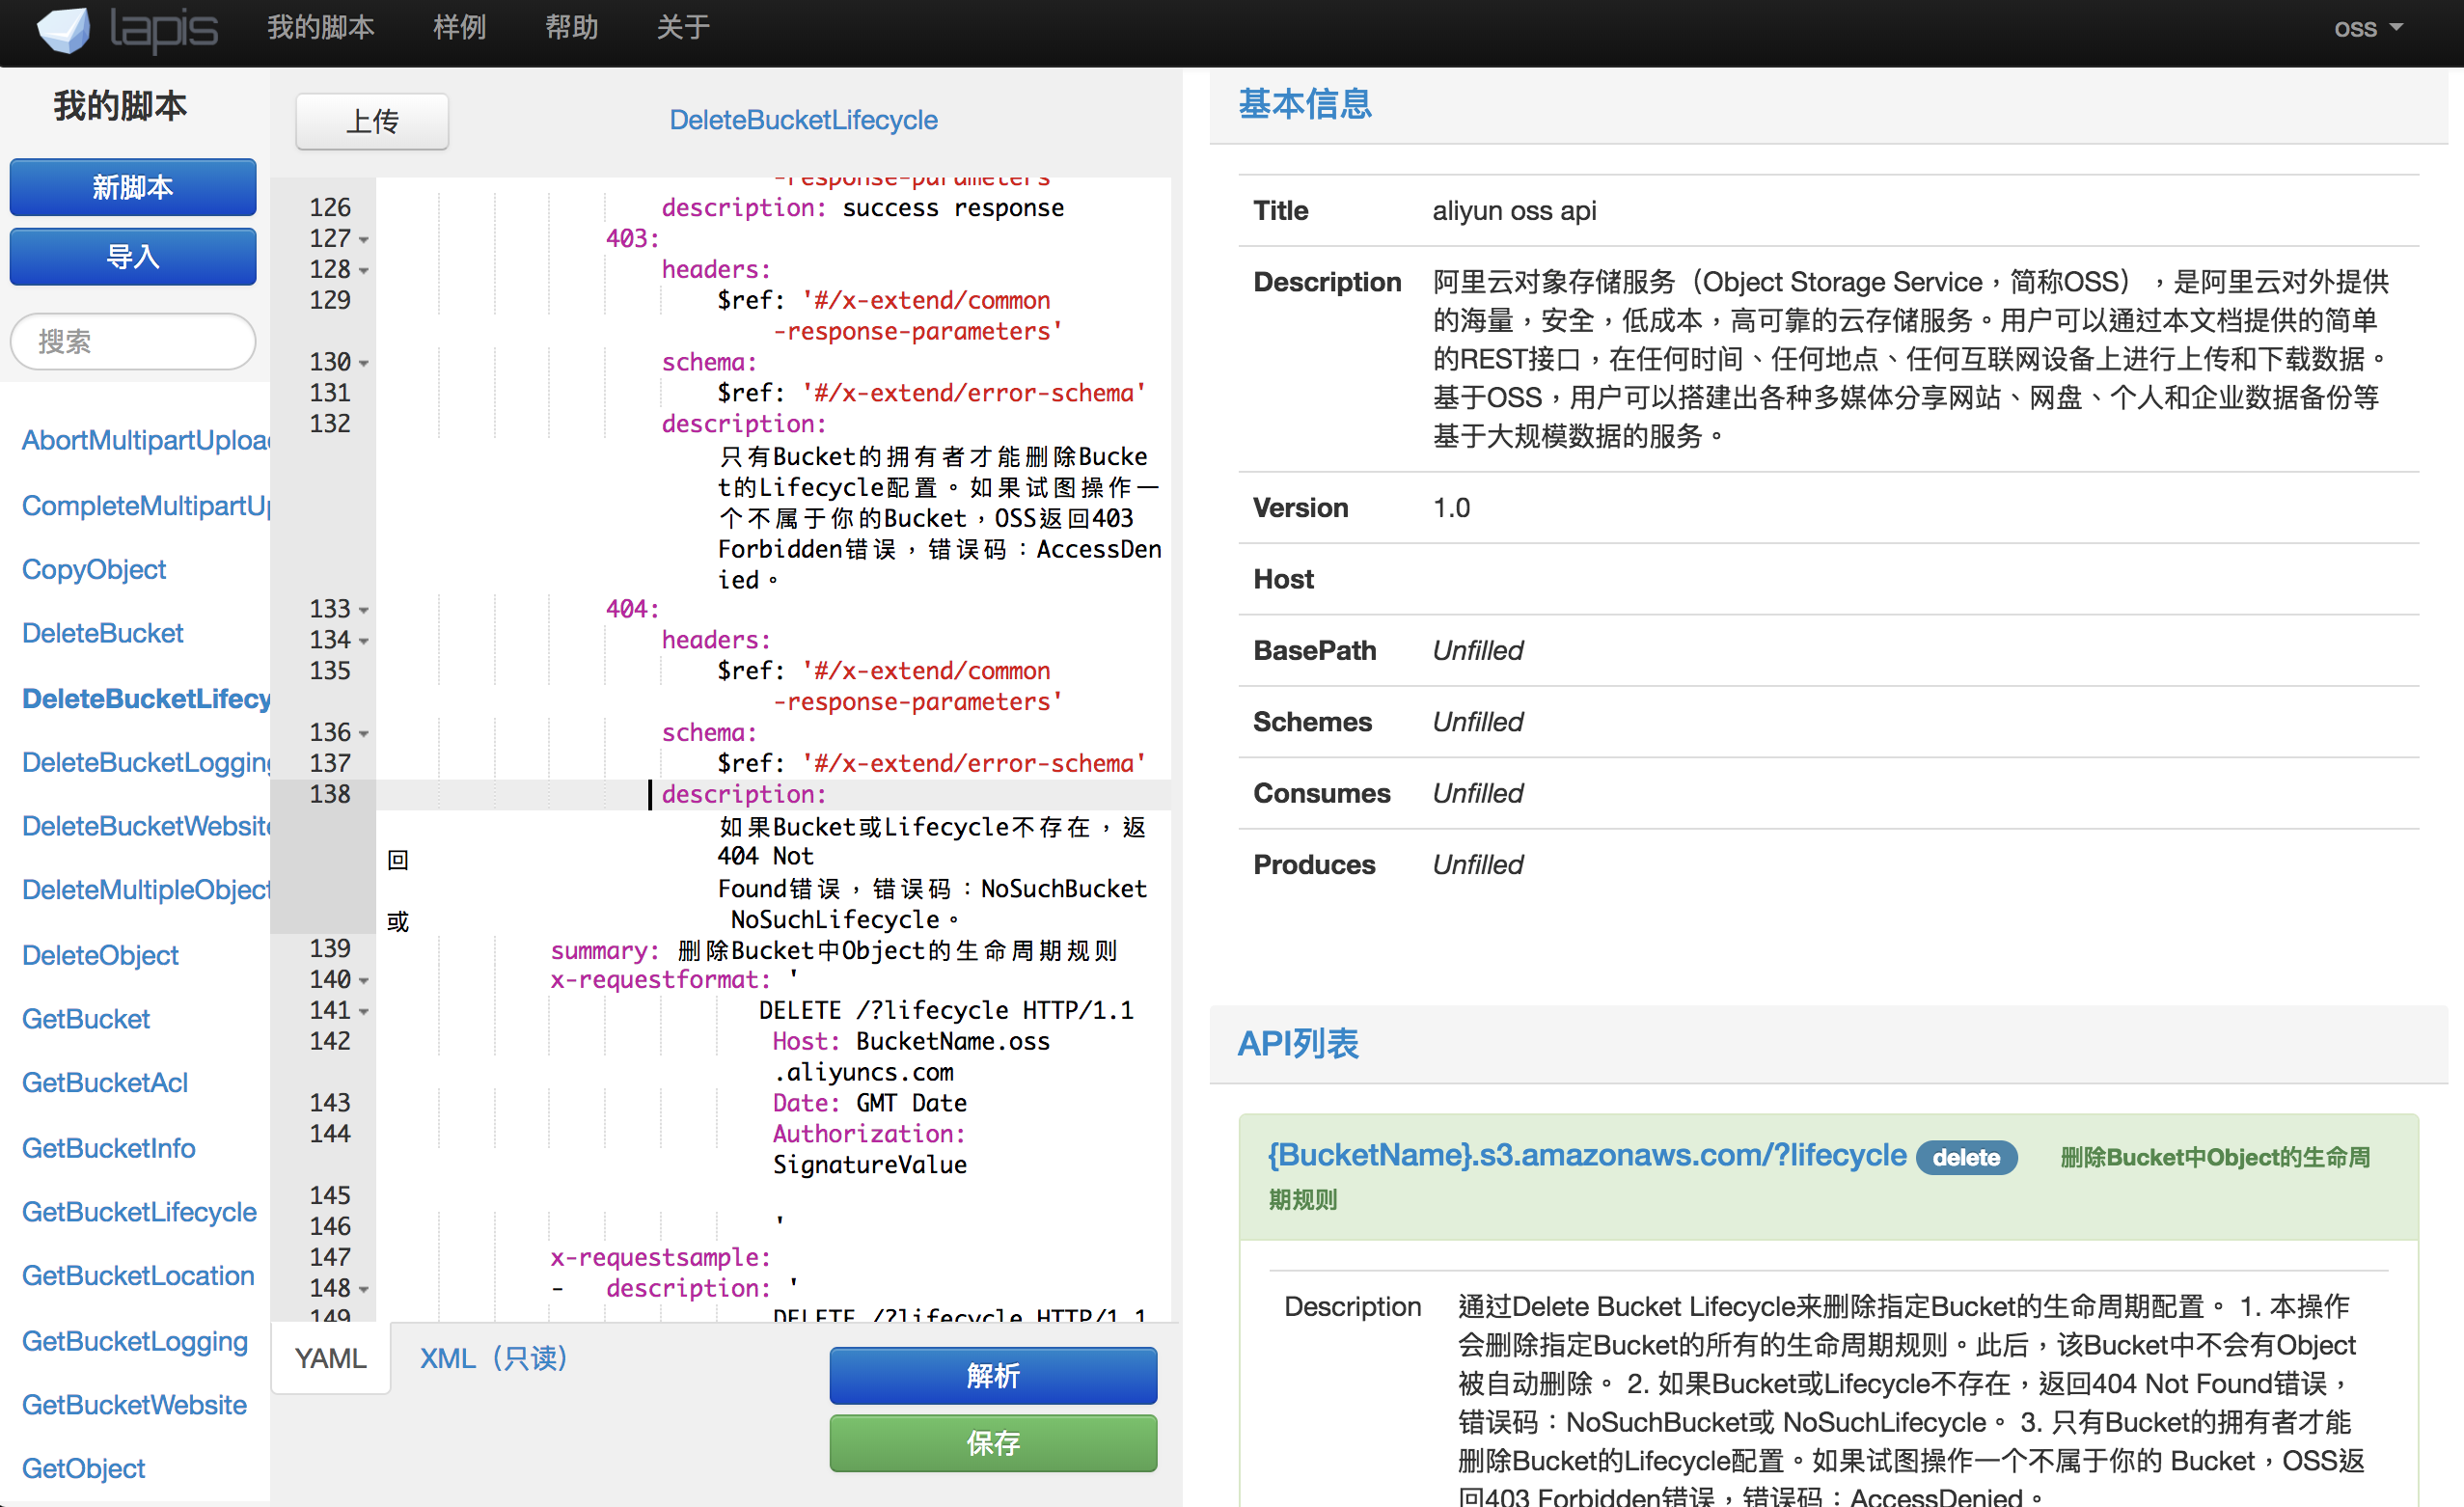
\includegraphics[width=200pt]{frontend_screenshot.png}
                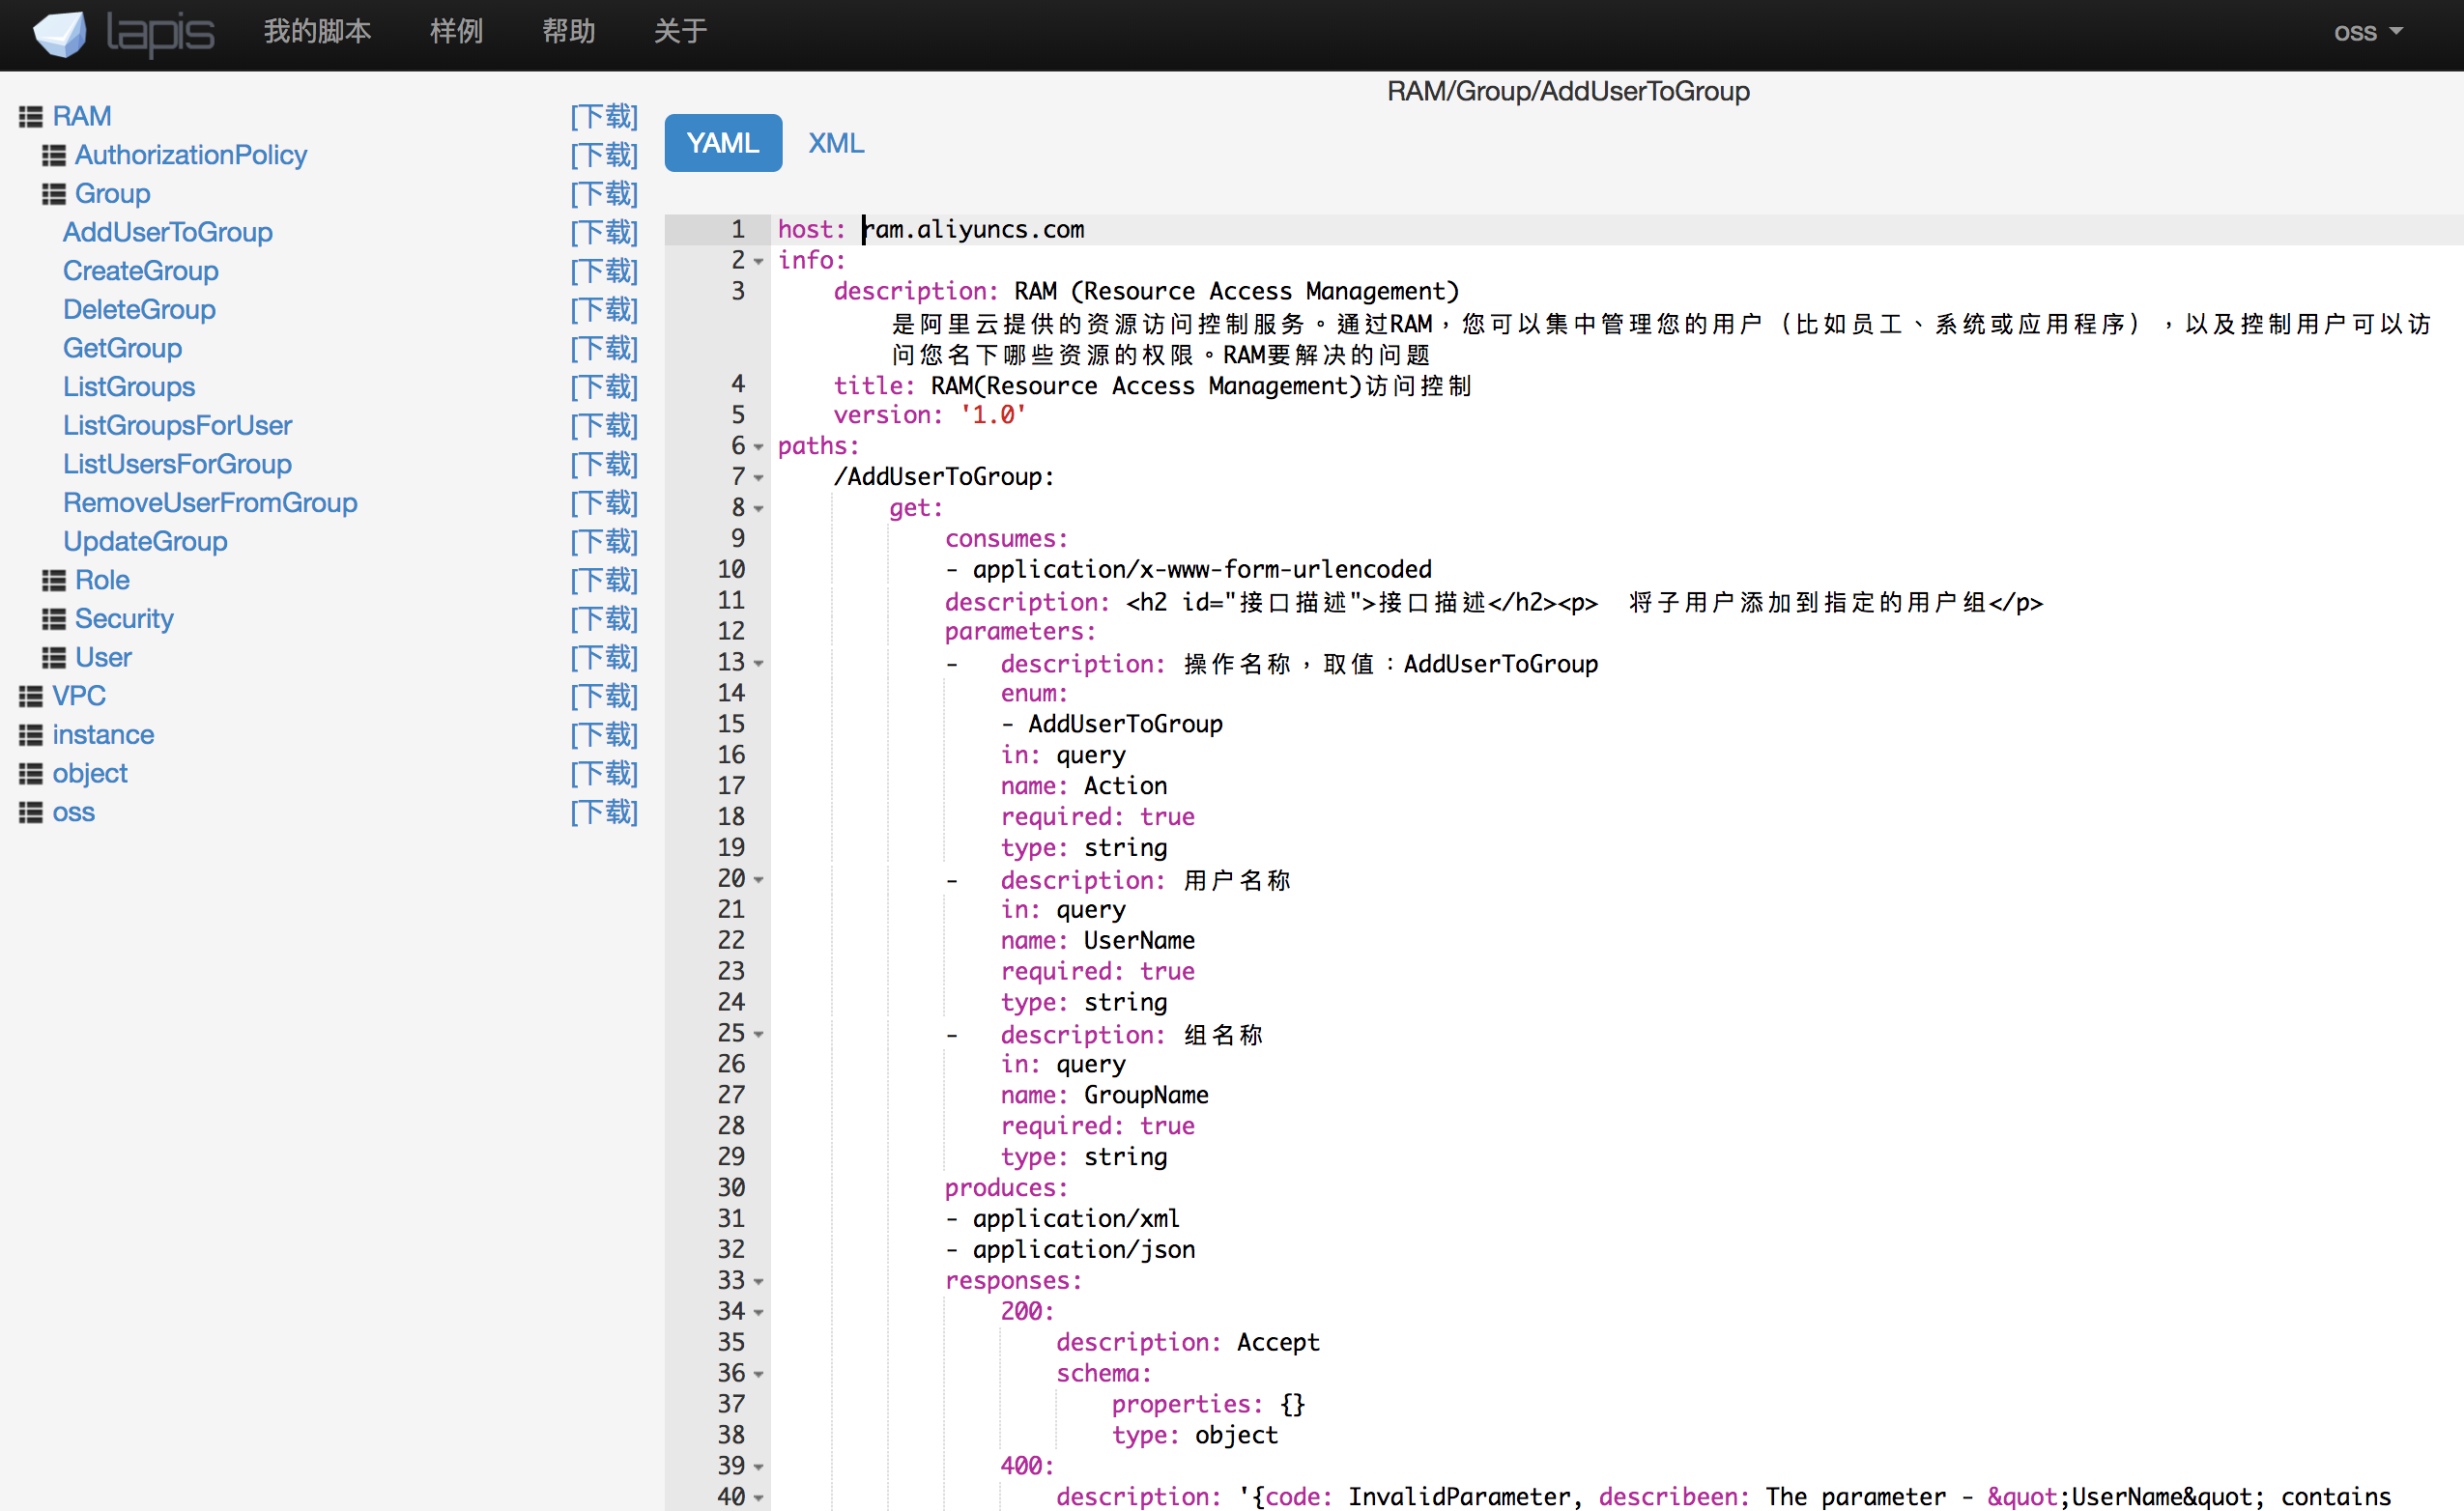
\includegraphics[width=200pt]{frontend_screenshot2.png}
                \caption{Web端脚本编辑系统前端截图. 通过此系统, 用户可以在线进行脚本的编辑与上传, 编辑时, 系统对API脚本进行实时解析, 以类似于API使用手册的形式展示脚本内容.}
                \label{fig:frontend_screenshot}
            \end{figure}
            
            此web编辑系统的后端采用Python语言和Django框架, 前端采用JQuery和Bootstrap库. 直接依托文件系统实现了用户和脚本托管功能, 没有数据库依赖, 十分轻量, 适合部署作为企业测试部门内部服务或单机使用.
        
            \label{sec:scenario_gui_edit}
            此外, 场景模型基于自动机模型, 故场景脚本不适于采用直接撰写的形式, 而适于用有向图表示, 并在图形化界面中拖拽生成\cite{junyiw17}. 开发创建场景模型的图形化界面将明显提高场景脚本的生成效率, 是未来可进一步研究的方向.
            
        % extended version
		% \subsection{*桌面端测试管理系统}


